\let\negmedspace\undefined
\let\negthickspace\undefined
\documentclass[journal]{IEEEtran}
\usepackage[a5paper, margin=10mm, onecolumn]{geometry}
%\usepackage{lmodern} % Ensure lmodern is loaded for pdflatex
\usepackage{tfrupee} % Include tfrupee package
\setlength{\headheight}{1cm} % Set the height of the header box
\setlength{\headsep}{0mm}     % Set the distance between the header box and the top of the text
\usepackage{gvv-book}
\usepackage{gvv}
\usepackage{cite}
\usepackage{amsmath,amssymb,amsfonts,amsthm}
\usepackage{algorithmic}
\usepackage{graphicx}
\usepackage{textcomp}
\usepackage{xcolor}
\usepackage{txfonts}
\usepackage{listings}
\usepackage{enumitem}
\usepackage{mathtools}
\usepackage{gensymb}
\usepackage{comment}
\usepackage[breaklinks=true]{hyperref}
\usepackage{tkz-euclide} 
\usepackage{listings}
% \usepackage{gvv}                                        
\def\inputGnumericTable{}                                 
\usepackage[latin1]{inputenc}                                
\usepackage{color}                                            
\usepackage{array}                                            
\usepackage{longtable}                                       
\usepackage{calc}                                             
\usepackage{multirow}                                         
\usepackage{hhline}                                           
\usepackage{ifthen}                                           
\usepackage{lscape}
\usepackage{float}
\begin{document}

\bibliographystyle{IEEEtran}
\vspace{3cm}

\title{9-9.5-5}
\author{EE24BTECH11050 - Pothuri Rahul}
% \maketitle
% \newpage
% \bigskip
{\let\newpage\relax\maketitle}

\renewcommand{\thefigure}{\theenumi}
\renewcommand{\thetable}{\theenumi}
\setlength{\intextsep}{10pt} % Space between text and floats


\numberwithin{equation}{enumi}
\numberwithin{figure}{enumi}
\renewcommand{\thetable}{\theenumi}
\textbf{Question}:\\
Find the area bounded by the curves $(x-1)^2 + y^2 = 1$ and $x^2 + y^2 = 1$.  \\
\solution \\
\begin{figure}[h]
    \centering
    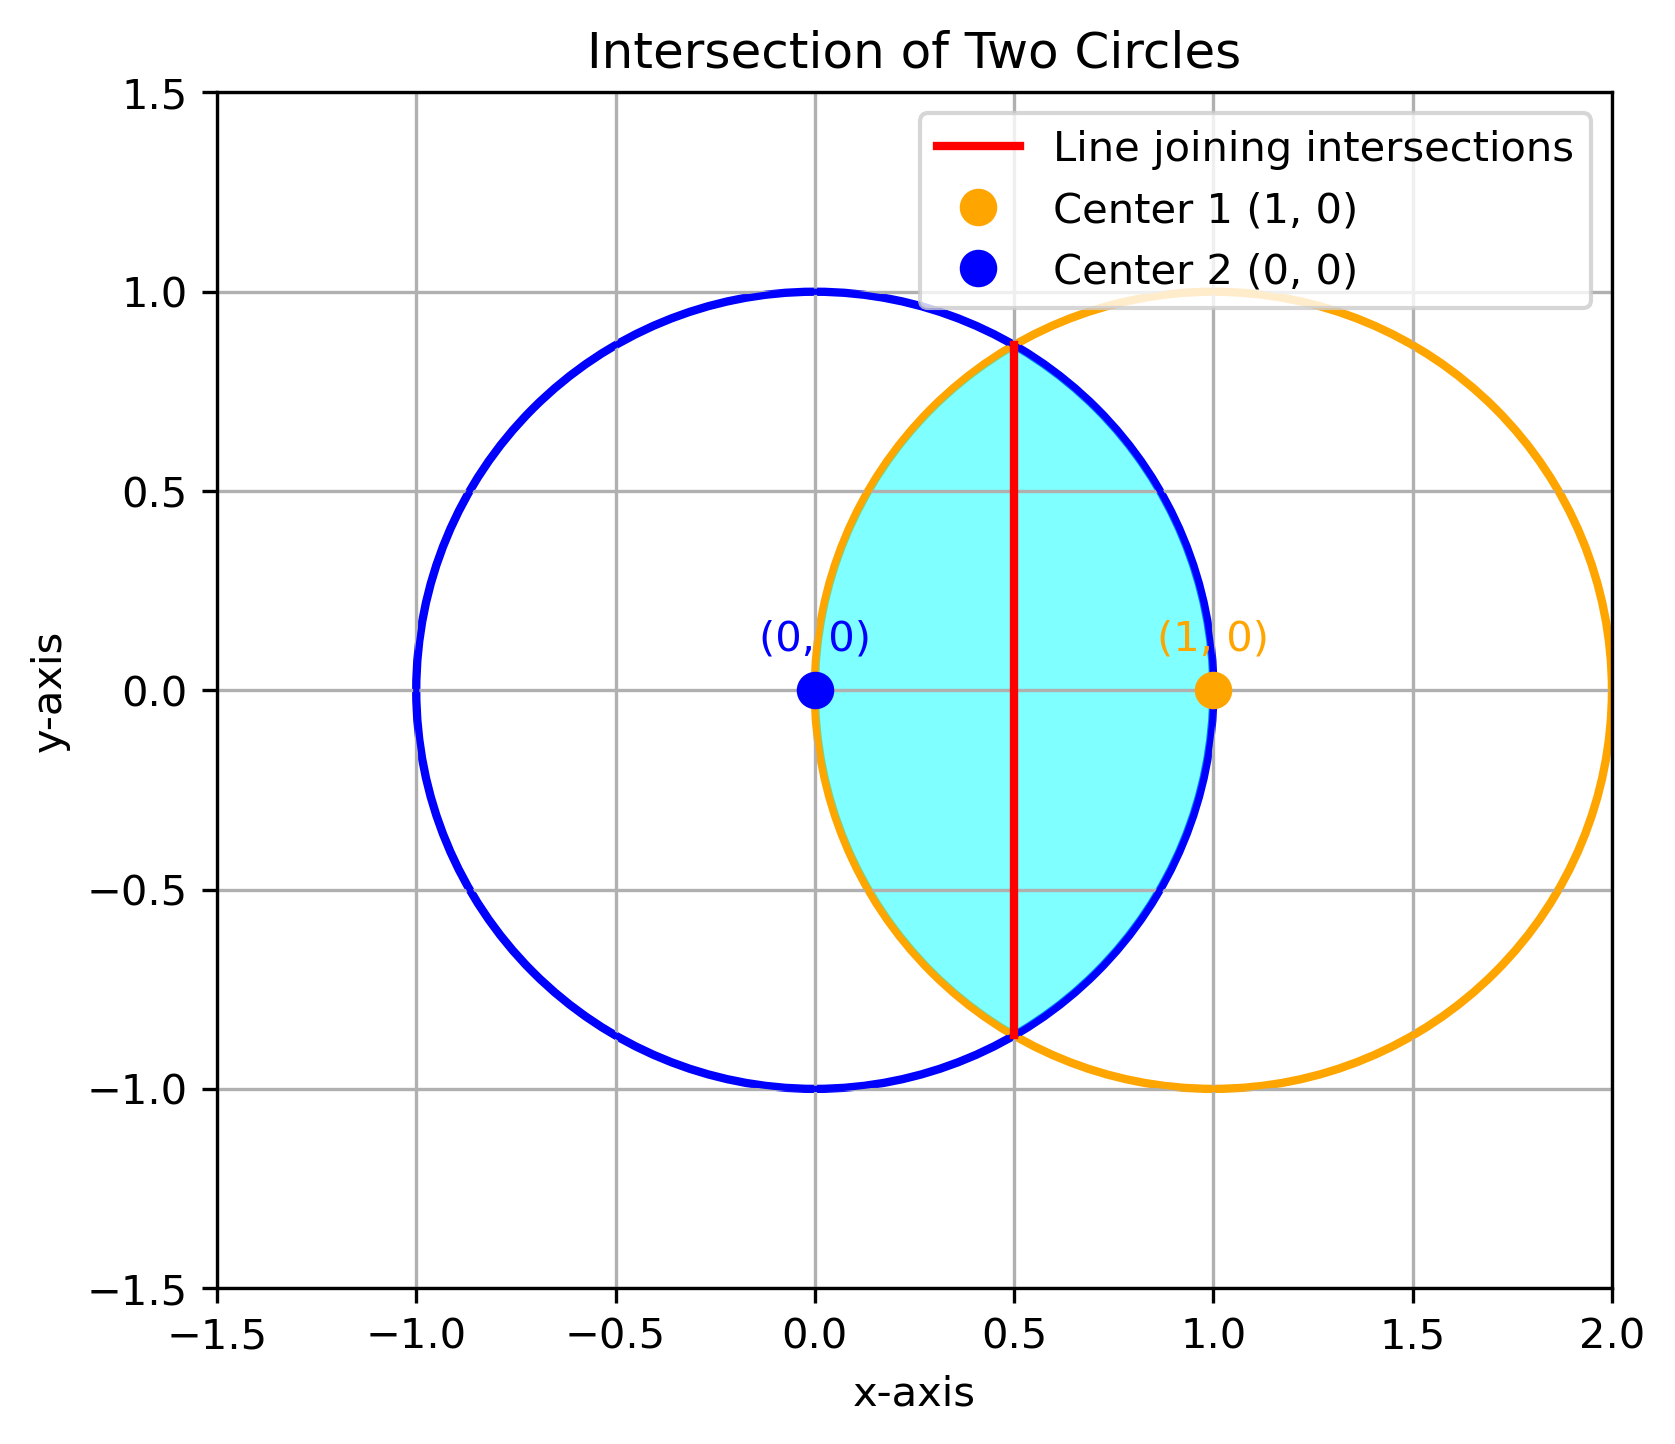
\includegraphics[width=0.6\textwidth]{fig.png}
    \caption{Intersection of the circles.}
\end{figure}

The intersection of two conics with parameters $V_i$ , $u_i$ , $f_i$ , $i = 1, 2$ is defined as
\begin{align}
      x^T\brak{V_1+\mu V_2}x+2\brak{u_1+\mu u_2}^Tx+\brak{f_1+\mu f_2}=0 \label{1}
\end{align}
 \eqref{1} represents a pair of stright lines if 
\begin{align}
\left| \begin{array}{cc}
V_1+\mu V_2 & u_1+\mu u_2 \\
\brak{u_1+\mu u_2}^T & f_1+\mu f_2
\end{array} \right| =0 \label{2}
\end{align}
The equation of line is
\begin{align}
x=h+\kappa m \label{3}
\end{align}
The conic parameters for the two circles can be expressed as
 \begin{align}
V_1 = \myvec{1 & 0 \\ 0 & 1}, \ u_1 = \myvec{ -1 \\ 0}, \ f_1 = 0, \label{4}
 \end{align}
 \begin{align}
V_2 = \myvec{1 & 0 \\ 0 & 1}, \ u_2 = \myvec{0 \\ 0}, \ f_2 = -1. \label{5}
 \end{align}
On substituting from \eqref{4} and \eqref{5} in \eqref{2}, we obtain
\begin{align}
\left| \begin{array}{ccc}
1 + \mu & 0 & -1 \\ 0 & 1 + \mu & 0 \\ -1 & 0 & -\mu 
\end{array} \right| = 0 \label{6}
\\
 \brak{1+\mu} \brak{1+\mu} \brak{-\mu}+\brak{1+\mu} =0 \label{7}
  \end{align}
yielding
 \begin{align}
\mu = -1. \label{8}
 \end{align}
Substituting \eqref{4} and \eqref{5} in \eqref{1}, we obtain
 \begin{align}
x^T \myvec{ 0 & 0 \\ 0 & 1} x + 2 \myvec{ -1 \\ 0}^T \myvec{ x \\ y} + 1 = 0 \\  
 \myvec{x & y} \myvec{0 & 0 \\ 0 & 1} \myvec{x \\ y}+2 \myvec{-1 & 0} \myvec{x \\ y}+1=0 \label{10}
 \end{align}
 \begin{align}
\Rightarrow (-2)(x-1) = 1 \quad \Rightarrow x = \frac{1}{2}. \label{11}
 \end{align}
Therefore the intersection of the two circles is a line with parameters
 \begin{align}
m = \myvec{0 \\ 1}, \ h = \myvec{\frac{1}{2} \\ 0}. \label{12}
 \end{align}

 The intersection parameters of the chord with the first circle in is obtained by substituting line equation in the conic equation.

we get $\kappa$ as following 

    \begin{multline}
\kappa_i = \frac{1}
{
m^{\top}Vm
}
\lbrak{-m^{\top}\brak{Vh+u}}
%\\
\pm
%{\small
\rbrak{\sqrt{
\sbrak{
m^{\top}\brak{Vh+u}
}^2
	-\text{g}
\brak
{h
%\vec{h}^{\top}\vec{V}\vec{h} + 2\vec{u}^{\top}\vec{h} +f
}
\brak{m^{\top}Vm}
}
}
%}
\label{13}
\end{multline}

Yielding
 \begin{align}
\kappa_i = \pm \frac{\sqrt{3}}{2}. \label{14}
 \end{align}
Hence the points of intersection are obtained from \eqref{2} as
 \begin{align}
x_1 = \left( \frac{1}{2}, \frac{\sqrt{3}}{2} \right), \quad x_2 = \left( \frac{1}{2}, -\frac{\sqrt{3}}{2} \right). \label{15}
 \end{align}
The desired area of the region is given as
 \begin{align}
2 \left( \int_0^{1/2} \sqrt{1 - (x - 1)^2} dx + \int_0^{1/2} \sqrt{1 - x^2} dx \right) \label{16}
 \end{align}
 \begin{align}
= 2 \left[ \frac{1}{2} \left( x - 1 \right) \sqrt{1 - (x - 1)^2} + \frac{1}{2} \sin^{-1}(x - 1) \right]_0^{1/2} + 2 \left[ \frac{1}{2} x \sqrt{1 - x^2} + \frac{1}{2} \sin^{-1}(x) \right]_0^{1/2} \label{17}
 \end{align}
 \begin{align}
= \frac{2\pi}{3} - \frac{\sqrt{3}}{2}. \label{18}
 \end{align}
 \\
 
 \begin{table}[h!]
    \centering
    \begin{tabular}[12pt]{|c|c|c|}
     \hline
     {parameter} & {discription} & {value}\\
     \hline
     $x_1$ & first intersection point & $\left( \frac{1}{2}, \frac{\sqrt{3}}{2} \right)$ \\
     \hline
     $x_2$ & second intersection point & $\left( \frac{1}{2}, -\frac{\sqrt{3}}{2} \right)$ \\
     \hline
     $V_1$ & \myvec{1-e_1^2 & 0 \\ 0 & 1} & \myvec{1 & 0 \\ 0 & 1}\\
     \hline
     $V_2$ & \myvec{1-e_2^2 & 0 \\ 0 & 1} & \myvec{1 & 0 \\ 0 & 1}\\
     \hline
     $c_1$ & centre of first circle& \myvec{1 \\ 0}\\
     \hline
     $u_1$ & -$c_1$ & \myvec{-1 \\ 0}\\
     \hline
     $c_2$ & centre of second circle& \myvec{0 \\ 0}\\
     \hline
     $u_2$ & -$c_2$ & \myvec{0 \\ 0}\\
     \hline
     $r_1$ & radius of first circle & i \\
     \hline
     $f_1$ & $\lVert u_1 \rVert^2 - r_1^2$ & 0 \\
     \hline
     $r_2$ & radius of second circle & 1\\
     \hline
     $f_2$ & $\lVert u_2 \rVert^2 - r_2^2$ & -1 \\
     \hline 
    $m$ & Slope of the line & \myvec{0 \\ 1}\\
    \hline
    $h$ & Intercept of the line & \myvec{\frac{1}{2} \\ 0} \\
    \hline
    $k_1$ &Parameter of first line & $\frac{\sqrt{3}}{2}$ \\
    \hline
    $k_2$ &Parameter of second line & - $\frac{\sqrt{3}}{2}$ \\
    \hline
     
\end{tabular}
    \caption{Parameters used}
    \label{tab:9.5-5}
\end{table}
\\

\end{document}
